\documentclass[semifinal]{cpecmu}

%% This is a sample document demonstrating how to use the CPECMU
%% project template. If you are having trouble, see "cpecmu.pdf" for
%% documentation.

\projectNo{P019-2}
\acadyear{2023}

\titleTH{แพลตฟอร์มดิจิทัลสำหรับการตรวจคัดกรองและเฝ้าระวังการเกิดรอยโรคก่อนมะเร็งและมะเร็งช่องปาก}
\titleEN{Digital Platform for Detecting and Analyzing Oral Potentially Malignant Disorders and Oral Cancer}

\author{นายชาญชัย ไชยสลี}{Chanchai Chaisalee}{630610726}
\author{นายเทวฤทธิ์ สมฤทธิ์}{Tewarad Somrad}{630610731}

\cpeadvisor{patiwet}
\cpecommittee{dome}
\cpecommittee{sansanee}

%% Some possible packages to include:
\usepackage[final]{graphicx} % for including graphics

\usepackage{float}%load this into your preamble

%% Add bookmarks and hyperlinks in the document.
\PassOptionsToPackage{hyphens}{url}
\usepackage[colorlinks=true,allcolors=Blue4,citecolor=red,linktoc=all]{hyperref}
\def\UrlLeft#1\UrlRight{$#1$}

%% Needed just by this example, but maybe not by most reports
\usepackage{afterpage} % for outputting
\usepackage{pdflscape} % for landscape figures and tables. 

%% Some other useful packages. Look these up to find out how to use
%% them.
% \usepackage{natbib}    % for author-year citation styles
% \usepackage{txfonts}
% \usepackage{appendix}  % for appendices on a per-chapter basis
% \usepackage{xtab}      % for tables that go over multiple pages
% \usepackage{subfigure} % for subfigures within a figure
% \usepackage{pstricks,pdftricks} % for access to special PostScript and PDF commands
% \usepackage{nomencl}   % if you have a list of abbreviations

%% if you're having problems with overfull boxes, you may need to increase
%% the tolerance to 9999
% \tolerance=9999

\bibliographystyle{plain}
% \bibliographystyle{IEEEbib}

% \renewcommand{\topfraction}{0.85}
% \renewcommand{\textfraction}{0.1}
% \renewcommand{\floatpagefraction}{0.75}

%% Example for glossary entry
%% Need to use glossary option
%% See glossaries package for complete documentation.
\ifglossary
  \newglossaryentry{lorem ipsum}{
    name=lorem ipsum,
    description={derived from Latin dolorem ipsum, translated as ``pain itself''}
  }
\fi

%% Uncomment this command to preview only specified LaTeX file(s)
%% imported with \include command below.
%% Any other file imported via \include but not specified here will not
%% be previewed.
%% Useful if your report is large, as you might not want to build
%% the entire file when editing a certain part of your report.
% \includeonly{chapters/intro,chapters/background}

\begin{document}
\maketitle
\makesignature

\ifproject
\begin{abstractTH}

แพลตฟอร์มดิจิทัลสำหรับการตรวจคัดกรองและเฝ้าระวังการเกิดรอยโรคก่อนมะเร็งและมะเร็งช่องปาก 
เป็นเว็บแอปพลิเคชั่นสำหรับรองรับระบบปัญญาประดิษฐ์ (AI) 
เพื่อตรวจคัดกรองและเฝ้าระวังการเกิดรอยโรคก่อนมะเร็งและมะเร็งช่องปาก (Digital Platform for Detecting and Analyzing Oral Potentially Malignant Disorders and Oral Cancer) เบื้องต้นได้ด้วยตนเอง 
กลุ่มผู้ใช้งานของดิจิทัลแพลตฟอร์มนี้จะเป็นทันตแพทย์และประชาชนทั่วไป โดยการยืนยันผลการตรวจของระบบปัญญาประดิษฐ์จะถูกยืนยันผลจากทันตแพทย์ที่เข้าร่วมโครงการ 
เมื่อตรวจสอบพบว่ามีรอยโรคจริงก็ดำเนินการรักษาในขั้นต่อไป

% การเขียนรายงานเป็นส่วนหนึ่งของการทำโครงงานวิศวกรรมคอมพิวเตอร์
% เพื่อทบทวนทฤษฎีที่เกี่ยวข้อง อธิบายขั้นตอนวิธีแก้ปัญหาเชิงวิศวกรรม และวิเคราะห์และสรุปผลการทดลองอุปกรณ์และระบบต่างๆ
% \enskip อย่างไรก็ดี การสร้างรูปเล่มรายงานให้ถูกรูปแบบนั้นเป็นขั้นตอนที่ยุ่งยาก
% แม้ว่าจะมีต้นแบบสำหรับใช้ในโปรแกรม Microsoft Word แล้วก็ตาม
% แต่นักศึกษาส่วนใหญ่ยังคงค้นพบว่าการใช้งานมีความซับซ้อน และเกิดความผิดพลาดในการจัดรูปแบบ กำหนดเลขหัวข้อ และสร้างสารบัญอยู่
% \enskip ภาควิชาวิศวกรรมคอมพิวเตอร์จึงได้จัดทำต้นแบบรูปเล่มรายงานโดยใช้ระบบจัดเตรียมเอกสาร
% \LaTeX{} เพื่อช่วยให้นักศึกษาเขียนรายงานได้อย่างสะดวกและรวดเร็วมากยิ่งขึ้น
\end{abstractTH}

\begin{abstract}

Digital Platform for Detecting and Analyzing Oral Potentially Malignant Disorders and Oral Cancer is web application integrated with AI
 for self detecting oral potentially malilgnant disorders and oral cancer. User group are dentist and general public.
  AI analyzed result will confirmed by dentist participating in the project. 
  If result is verified to be disorders, proceed with treatment in the next step.
% The abstract would be placed here. It usually does not exceed 350 words
% long (not counting the heading), and must not take up more than one (1) page
% (even if fewer than 350 words long).

% Make sure your abstract sits inside the \texttt{abstract} environment.
\end{abstract}

\iffalse
\begin{dedication}
This document is dedicated to all Chiang Mai University students.

Dedication page is optional.
\end{dedication}
\fi % \iffalse

\begin{acknowledgments}

    โครงงานนี้จะไม่สําเร็จลุล่วงลงได้ ถ้าหากไม่ได้รับความกรุณาจาก รศ.ดร.ปฏิเวธ วุฒิสารวัฒนา อาจารย์ที่ปรึกษาโครงงาน ที่ได้สละเวลาส่วนตัวมาให้ความช่วยเหลือแก่โครงงานนี้ โดยได้ให้คําเสนอแนะ แนวคิด ช่องทางการหาความรู้ที่จําเป็นในการทําเว็บแอพลิเคชัน 
    ตลอดจนช่วยตรวจสอบแก้ไขข้อบกพร่องต่างๆ มาโดยตตลอด รวมถึง ผศ.โดม โพธิกานนท์ และ รศ.ดร. ศันสนีย์ เอื้อพันธ์วิริยะกุล ที่ให้คําปรึกษา คําแนะนํา 
    จนทําให้โครงงานนี้มีความสมบูรณ์มากที่สุด
    
    ขอบคุณคณะวิศวกรรมศาสตร์ มหาวิทยาลัยเชียงใหม่ ที่ให้สถานที่ในการทําโครงงาน ทั้งห้องภาควิชา
    วิศวกรรมคอมพิวเตอร์ และสถานที่ต่างๆในภาควิชา และยังให้การสนับสนุนทางด้านงบประมาณ อุปกรณ์
    ต่างๆ ที่จําเป็นต่อการทําโครงงาน
    
    ขอขอบพระคุณผู้ปกครอง เพื่อนและรุ่นพี่ทุกคน ที่ให้คําปรึกษา คําแนะนํา เเละคอยเป็นกําลังใจ
    ให้ตลอดมา ซึ่งเป็นแรงผลักดันให้แก่ผู้จัดทํามีความตั้งใจและมุ่งมั่นในการทํางาน จนโครงงานที่ความสมบูรณ์
    มากที่สุด
    
    นอกจากนี้ผู้จัดทําขอขอบพระคุณอีกหลายๆท่านที่ไม่ได้กล่าวถึง ณ ที่นี้ ที่ได้ให้ความช่วยเหลือตลอดมา
    และสุดท้ายนี้ หากโครงงานนี้มีข้อผิดพลาดประการใด ผู้จัดทําขออภัยมา ณ ที่นี้ และพร้อมน้อมรับด้วยความ
    ยินดี
\texttt{acknowledgment} environment.

\acksign{2020}{5}{25}
\end{acknowledgments}%
\fi % \ifproject

\contentspage

\ifproject
\figurelistpage

\tablelistpage
\fi % \ifproject

% \abbrlist % this page is optional

% \symlist % this page is optional

% \preface % this section is optional


\pagestyle{empty}\cleardoublepage
\normalspacing \setcounter{page}{1} \pagenumbering{arabic} \pagestyle{cpecmu}

\chapter{\ifenglish Introduction\else บทนำ\fi}

\section{\ifenglish Project rationale\else ที่มาของโครงงาน\fi}

ในปัจจุบันปัญหาด้านสุขภาพของประชากรมีแนวโน้มจะสูงขึ้นเรื่อย ๆ ประกอบกับการเข้าสู่สังคมสูงวัยของประชากร ปัญหาสุขภาพจึงเป็นปัญหาที่สำคัญ ซึ่งส่งผลกระทบต่อชีวิตของประชากรโดยส่วนมาก มะเร็งช่องปากเป็นมะเร็งชนิดหนึ่งที่พบมากในกลุ่มประชากรที่มีอายุตั้งแต่ 40 ปี ขึ้นไป ที่มีประวัติด้านการสูบบุหรี่ และ/หรือดื่มแอลกอฮอล์ และเคี้ยวหมาก ซึ่งการตรวจสอบรอยโรคในระยะแรกอาจทำได้ยากโดยทั่วไปและหากปล่อยเป็นระยะเวลานานเกินไปอาจทำให้รอยโรคลุกลามเป็นมะเร็งได้ในที่สุด 

คณะผู้จัดทำมีความสนใจในเรื่องนี้ จึงได้จัดทำดิจิทัลแพลตฟอร์มเพื่อรองรับระบบปัญญาประดิษฐ์ (AI) เพื่อใช้ในการตรวจสอบและคัดกรองรอยโรคก่อนมะเร็งช่องปากและมะเร็งช่องปาก ที่ใช้ร่วมกับการประเมินจากทันตแพทย์ผู้เชี่ยวชาญ คณะผู้จัดทำจึงได้นำเสนอการพัฒนาเว็บแอปพลิเคชัน ซึ่งเป็นแพลตฟอร์มดิจิทัลสำหรับรองรับระบบปัญญาประดิษฐ์ (AI) เพื่อตรวจคัดกรองและเฝ้าระวังการเกิดรอยโรคก่อนมะเร็งและมะเร็งช่องปาก (Digital Platform for Detecting and Analyzing Oral Potentially Malignant Disorders and Oral Cancer) โดยกลุ่มผู้ใช้งานของดิจิทัลแพลตฟอร์มนี้จะเป็นทันตแพทย์ทั่วประเทศและประชากรทั่วไปที่มีความสนใจในการนำดิจิทัลแพลตฟอร์มนี้ไปใช้ 

คณะผู้จัดทำหวังว่า ดิจิทัลแพลตฟอร์มนี้จะส่งผลให้ทันตแพทย์ทั่วประเทศสามารถตรวจหามะเร็งช่องปากได้อย่างรวดเร็ว และเป็นเครื่องมือหนึ่งที่จะช่วยแก้ไขปัญหาด้านสุขภาพของประชากรโดยเฉพาะมะเร็งช่องปากได้อย่างมีประสิทธิภาพ
\section{\ifenglish Objectives\else วัตถุประสงค์ของโครงงาน\fi}
\begin{enumerate}
    \item พัฒนาเว็บแอปพลิเคชันเพื่อรองรับระบบปัญญาประดิษฐ์(AI)
    \item พัฒนาเว็บแอปพลิเคชันเพื่อตรวจคัดกรองและเฝ้าระวังการเกิดรอยโรคก่อนมะเร็งและมะเร็งช่องปาก
\end{enumerate}

\section{\ifenglish Project scope\else ขอบเขตของโครงงาน\fi}

\subsection{\ifenglish Hardware scope\else ขอบเขตด้านฮาร์ดแวร์\fi}
โครงการนี้ต้องการฮาร์ดแวร์ต่อไปนี้ จึงจะสามารถใช้งานได้อย่างมีประสิทธิภาพ

• คอมพิวเตอร์ส่วนบุคคลหรือโทรศัพท์มือถือที่สามารถใช้งานเว็บเบราว์เซอร์ได
\subsection{\ifenglish Software scope\else ขอบเขตด้านซอฟต์แวร์\fi}
โครงการนี้ต้องการซอฟต์แวร์ต่อไปนี้ จึงจะสามารถใช้งานได้อย่างมีประสิทธิภาพ

• สามารถใช้งานเว็บไซต์บนระบบปฏิบัติการทั่วไปได้ เช่น Windows, macOS, Linux, Android, iOS และอื่น ๆ

\section{\ifenglish Expected outcomes\else ประโยชน์ที่ได้รับ\fi}
ผู้ใช้งาน

• สามารถใช้งานเว็บแอปพลิเคชันเพื่อตรวจคัดกรองและเฝ้าระวังการเกิดรอยโรคก่อนมะเร็งและมะเร็งช่อง
ปากได้

• สามารถเข้าถึงการรักษาทางการแพทย์ได้อย่างรวดเร็ว หลังจากที่ผู้ใช้งานได้รับการตรวจคัดกรองและ
เฝ้าระวังการเกิดรอยโรคก่อนมะเร็งและมะเร็งช่องปากโดยเว็บแอปพลิเคชัน

\noindent ผู้พัฒนา

• ได้รับความรู้และความเข้าใจในการพัฒนาเว็บแอปพลิเคชันเพื่อรองรับระบบปัญญาประดิษฐ์(AI)

• ได้ฝึกทักษะในการพัฒนาเว็บแอปพลิเคชันเพื่อรองรับระบบปัญญาประดิษฐ์(AI)

• ได้ฝึกทักษะในการทํางานเป็นทีมและทักษะในการวิเคราะห์และแก้ไขปัญหาที่อาจเกิดขึ้นในการพัฒนา

\section{\ifenglish Technology and tools\else เทคโนโลยีและเครื่องมือที่ใช้\fi}

\subsection{\ifenglish Hardware technology\else เทคโนโลยีด้านฮาร์ดแวร์\fi}

\subsection{\ifenglish Software technology\else เทคโนโลยีด้านซอฟต์แวร์\fi}

• ภาษาโปรแกรมมิ่ง: JavaScript, Python, HTML, CSS

• ฐานข้อมูล: MySQL

• เครื่องมือและเทคโนโลยี: NextJS, Tailwind CSS, Git, GitHub, Minio
\section{\ifenglish Project plan\else แผนการดำเนินงาน\fi}

\begin{plan}{11}{2023}{2}{2024}
    \planitem{11}{2023}{1}{2024}{ศึกษาค้นคว้าเกี่ยวกับเทคโนโลยีที่เกี่ยวข้อง}
    \planitem{12}{2023}{12}{2023}{ออกแบบฟีเจอร์ที่จะเพิ่มในเว็บแอปพลิเคชัน}
    \planitem{1}{2024}{2}{2024}{พัฒนาฟีเจอร์ตามที่ได้ออกแบบไว้}
    \planitem{2}{2023}{2}{2024}{ทดสอบและปรับปรุง}
\end{plan}

\section{\ifenglish Roles and responsibilities\else บทบาทและความรับผิดชอบ\fi}

มีหน้าที่และความรับผิดชอบ ดังนี้

นายชาญชัย ไชยสลี รหัสนักศึกษา 630610726 รับผิดชอบในการศึกษาค้นคว้าเทคโนโลยีที่เกี่ยวข้อง,
ออกแบบโครงสร้างของเว็บแอปพลิเคชันและพัฒนาเว็บแอปพลิเคชัน

นายเทวฤทธิ์ สมฤทธิ์ รหัสนักศึกษา 630610731 รับผิดชอบในการศึกษาค้นคว้าเทคโนโลยีที่เกี่ยวข้อง,
ออกแบบโครงสร้างของเว็บแอปพลิเคชันและพัฒนาเว็บแอปพลิเคชัน


\section{\ifenglish%
Impacts of this project on society, health, safety, legal, and cultural issues
\else%
ผลกระทบด้านสังคม สุขภาพ ความปลอดภัย กฎหมาย และวัฒนธรรม
\fi}

โครงงานนี้จัดทำขึ้นเพื่อให้ประชาชนทั่วไปได้มีโอกาสเข้าถึงการรักษาได้มากยิ่งขึ้น เพิ่มโอกาสการรักาาสำเร็จให้สูงขั้นได้
ถ้าตรวจพบโรคได้เร็วพอ แต่ทั้งนี้ก็ต้องอาศัยความร่วมมือจากหน่วยงานทางการแพทย์ที่นำไปใช้งานจริง

\chapter{\ifenglish Background Knowledge and Theory\else ทฤษฎีที่เกี่ยวข้อง\fi}

\section{ด้านโครงสร้างเว็บแอปพลิเคชัน}

ในส่วนนี้จะอธิบายถึงโครงสร้างของเว็บแอปพลิเคชันที่ใช้ในการพัฒนา
\subsection{MVC Architecture}

MVC [1] เป็นตัวย่อของคําว่า Model View Controller ใช้เรียกรูปแบบการพัฒนาซอฟต์แวร์ที่มีโครงสร้างซึ่งแบ่งออกมาเป็น 3 ส่วนหลัก ตามตัวย่อของชื่อ รูปแบบการพัฒนาซอฟต์แวร์แบบ MVC ถูกนําไปใช้
ในขั้นตอนการพัฒนาหลากหลายภาษา เพราะ MVC เป็นเพียงหลักการออกแบบโปรแกรม (Design Pattern) รูปแบบหนึ่งเท่านั้น ซึ่งเป็นที่นิยมมาก ในการนํามาพัฒนาแอพพลิเคชั่นซอฟต์แวร์แต่ละแพลตฟอร์ม
และประยุกต์ใช้ในอีกหลาย ๆ ด้าน

\subsubsection{ส่วนของ Model (M)}
model คือส่วนของการเก็บรวบรวมข้อมูล ไม่ว่าข้อมูลนั้น ๆ จะถูกจัดเก็บในรูปแบบใดก็ตาม ในฐานข้อมูล
แบบเป็น Object Class หรือที่นิยมเรียกกันว่า VO ( Value Object ) หรือเก็บเป็นไฟล์ข้อมูลเลย เมื่อ

ข้อมูลถูกโหลดเข้ามาจากที่ต่าง ๆ และเข้ามายังส่วนของโมเดล ตัวโมเดลจะทําการจัดการตระเตรียมข้อมูลให้
เป็นรูปแบบที่เหมาะสม เพื่อรอการร้องขอข้อมูลจากส่วนของ Controller

\subsubsection{ส่วนของ View (V)}
view คือส่วนของการแสดงผล หรือส่วนที่จะปฏิสัมพันธ์กับผู้ใช้งาน ( User Interface ) หน้าที่ของ view
ในการเขียนโปรแกรมแบบ MVC คือคอยรับคําสั่งจากส่วนของ Controller และ End User เริ่มแรกเลยตัว
วิว อาจจะได้รับคําสั่งจาก Controller ให้แสดงผลหน้า Home และเมื่อผู้ใช้งานหน้าเว็บกดป่ ุมสั่งซื้อ View
จะส่งข้อมูลไปให้Controller เพื่อประมวลผลและแสดงบางอย่างจาก Action นั้น

\subsubsection{ส่วนของ Controller (C)}
controller คือส่วนของการเริ่มทํางาน และรับคําสั่ง โดยที่คําสั่งนั้นจะเกิดขึ้นในส่วนการติดต่อกับผู้ใช้งานคือ
view เมื่อผู้ใช้งานทําการ Interactive กับ UI view จะเกิดเหตุการณ์หรือข้อมูลบางอย่างขึ้น ตัววิวจะส่งข้อมูลนั้น มายัง controller ตัว controller จะทําการประมวลผลโดยบางคําสั่งอาจจะต้องไปติดต่อกับ model
ก่อน เพื่อทําการประมวลผลข้อมูลอย่างถูกต้องเรียบร้อยแล้วก็จะส่งไปยัง view เพื่อแสดงผลตามคําสั่งที่ end
user ร้องขอมา Controller จะทําหน้าที่เป็นตัวกลางระหว่าง Model และ View ให้ทํางานร่วมกันอย่างมี
ประสิทธิภาพและตรงกับ ความต้องการของ End User มากที่สุด
\subsection{RESTful API}

RESTful API [2] เป็นอินเทอร์เฟซที่ระบบคอมพิวเตอร์สองระบบใช้เพื่อแลกเปลี่ยนข้อมูลผ่านอินเทอร์เน็ตได้อย่างปลอดภัย แอปพลิเคชันทางธุรกิจส่วนใหญ่ต้องสื่อสารกับแอปพลิเคชันภายในอื่นๆ และของบุคคลที่สามเพื่อทํางานต่างๆ ตัวอย่างเช่น หากต้องการสร้างสลิปเงินเดือน ระบบบัญชีภายในของคุณต้องแบ่งปัน
ข้อมูลกับระบบธนาคารของลูกค้าเพื่อออกใบแจ้งหนี้และสื่อสารกับแอปพลิเคชันบันทึกเวลาปฏิบัติงานภายใน
โดยอัตโนมัติRESTful API ให้การสนับสนุนการแลกเปลี่ยนข้อมูลนี้เพราะเป็นระบบที่มีมาตรฐานการสื่อสารระหว่างซอฟต์แวร์ที่ปลอดภัย เสถียร และมีประสิทธิภาพ

\subsubsection{API (Application Programming Interface)}
ส่วนต่อประสานโปรแกรมประยุกต์(Application Programming Interface หรือ API) กําหนดกฎที่คุณ
ต้องปฏิบัติตามเพื่อสื่อสารกับระบบซอฟต์แวร์อื่น โดยนักพัฒนาเปิ ดเผยหรือสร้าง API เพื่อให้แอปพลิเคชัน
อื่นสามารถสื่อสารกับแอปพลิเคชันของตนได้ทางโปรแกรม ตัวอย่างเช่น แอปพลิเคชันบันทึกเวลาปฏิบัติงาน
แสดง API ที่ขอชื่อเต็มของพนักงานและช่วงวันที่ เมื่อได้รับข้อมูลนี้แล้ว ระบบจะประมวลผลบันทึกเวลาปฏิบัติงานของพนักงานเป็นการภายใน
 และส่งกลับจํานวนชั่วโมงที่ทํางานในช่วงวันที่ดังกล่าว ทั้งนี้คุณสามารถ
มองได้ว่า API เว็บเป็นเกตเวย์ระหว่างไคลเอ็นต์และทรัพยากรบนเว็บ

ไคลเอ็นต์ ไคลเอ็นต์คือผู้ใช้ที่ต้องการเข้าถึงข้อมูลจากเว็บ โดยไคลเอ็นต์อาจเป็นบุคคลหรือระบบซอฟต์แวร์ที่ใช้API ก็ได้ 
ตัวอย่างเช่น นักพัฒนาสามารถเขียนโปรแกรมที่เข้าถึงข้อมูลสภาพอากาศจากระบบสภาพ
อากาศ หรือคุณสามารถเข้าถึงข้อมูลเดียวกันจากเบราว์เซอร์เมื่อคุณเยี่ยมชมเว็บไซต์รายงานสภาพอากาศได้
โดยตรง

ทรัพยากร ทรัพยากรคือข้อมูลที่แอปพลิเคชันต่างๆ มอบให้แก่ไคลเอ็นต์ โดยทรัพยากรอาจเป็นรูปภาพ
วิดีโอ ข้อความ ตัวเลข หรือข้อมูลประเภทใดก็ได้ ทั้งนี้เครื่องคอมพิวเตอร์ที่มอบทรัพยากรให้แก่ไคลเอ็นต์นั้น
เรียกอีกอย่างว่าเซิร์ฟเวอร์ องค์กรต่างๆ ใช้API เพื่อแบ่งปันทรัพยากรและให้บริการเว็บในขณะที่ยังคงดูแล
รักษาความปลอดภัย การควบคุม และการรับรองความถูกต้องไปพร้อมกัน นอกจากนี้API ยังช่วยให้ลูกค้า
ระบุได้ว่าไคลเอ็นต์ใดสามารถเข้าถึงทรัพยากรภายในที่เฉพาะเจาะจงได้

\subsubsection{REST (Representational State Transfer)}

REST เป็นสถาปัตยกรรมซอฟต์แวร์ที่กําหนดเงื่อนไขว่า API ควรทํางานอย่างไร โดยแต่แรกเริ่มนั้น มีการ
สร้าง REST ขึ้นเพื่อเป็นแนวทางในการจัดการการสื่อสารบนเครือข่ายที่ซับซ้อน เช่น อินเทอร์เน็ต คุณสามารถใช้สถาปัตยกรรม REST เพื่อรองรับการสื่อสารที่มีประสิทธิภาพสูงและเชื่อถือได้ในทุกระดับ คุณยังสามารถใช้และปรับเปลี่ยนสถาปั ตยกรรมได้อย่างง่ายดาย โดยนําความสามารถในการมองเห็นและการเคลื่อน
ย้ายข้ามแพลตฟอร์มมาสู่ทุกระบบ API

นักพัฒนา API สามารถออกแบบ API ได้โดยใช้สถาปั ตยกรรมต่างๆ โดย API ที่เป็นไปตามรูปแบบสถาปัตยกรรม REST เรียกว่า REST API บริการเว็บที่ใช้สถาปัตยกรรม REST เรียกว่าบริการเว็บ RESTful
คําว่า RESTful API โดยทั่วไปหมายถึง API เว็บแบบ RESTful อย่างไรก็ตาม คุณสามารถใช้คําว่า REST
API และ RESTful API แทนกันได

\subsection{ระบบฐานข้อมูล (Database System)}

ระบบฐานข้อมูล (Database System) [3] คือ ระบบที่รวบรวมข้อมูลต่าง ๆ ที่เกี่ยวข้องกันเข้าไว้ด้วยกันอย่าง
มีระบบ มีความสัมพันธ์ระหว่างข้อมูลต่าง ๆ ที่ชัดเจน ในระบบฐานข้อมูลจะประกอบด้วยแฟ้มข้อมูลหลาย
แฟ้มที่มีข้อมูลเกี่ยวข้องสัมพันธ์กันเข้าไว้ด้วยกันอย่างเป็นระบบและเปิดโอกาสให้ผู้ใช้สามารถใช้งาน และดูแล
รักษาป้องกันข้อมูลเหล่านี้ได้อย่างมีประสิทธิภาพ โดยมีซอฟต์แวร์ที่เปรียบเสมือนสื่อกลางระหว่าง ผู้ใช้และ
โปรแกรมต่าง ๆ ที่เกี่ยวข้องกับการใช้ฐานข้อมูล เรียกว่า ระบบจัดการฐานข้อมูล หรือ DBMS (data base
management system)มีหน้าที่ช่วยให้ผู้ใช้เข้าถึงข้อมูลได้ง่ายสะดวกและมีประสิทธิภาพ การเข้าถึงข้อมูล
ของผู้ใช้อาจเป็นการสร้างฐานข้อมูล การแก้ไขฐานข้อมูล หรือการตั้งคําถามเพื่อให้ได้ข้อมูลมา โดยผู้ใช้ไม่จําเป็นต้องรับรู้เกี่ยวกับรายละเอียดภายในโครงสร้างของฐานข้อมูล

ประโยชน์ของฐานข้อมูล

1. ลดการเก็บข้อมูลที่ซํ้าซ้อน
ข้อมูลบางชุดที่อยู่ในรูปของแฟ้มข้อมูลอาจมีปรากฏอยู่หลาย ๆ แห่ง เพราะมีผู้ใช้ข้อมูลชุดนี้หลายคน
เมื่อใช้ระบบฐานข้อมูลแล้วจะช่วยให้ความซํ้าซ้อนของข้อมูลลดน้อยลง

2. รักษาความถูกต้องของข้อมูล
เนื่องจากฐานข้อมูลมีเพียงฐานข้อมูลเดียว ใน กรณีที่มีข้อมูลชุดเดียวกันปรากฏอยู่หลายแห่งในฐานข้อมูล ข้อมูลเหล่านี้จะต้องตรงกัน ถ้ามีการแก้ไขข้อมูลนี้ทุก ๆ แห่งที่ข้อมูลปรากฏอยู่จะแก้ไขให้ถูกต้อง
ตามกันหมดโดยอัตโนมัติด้วยระบบจัดการฐานข้อมูล

3. การป้องกันและรักษาความปลอดภัยให้กับข้อมูลทําได้อย่างสะดวก
การป้องกันและรักษาความปลอดภัยกับข้อมูลระบบฐานข้อมูลจะให้เฉพาะผู้ที่เกี่ยวข้องเท่านั้น ซึ่งก่อ
ให้เกิดความปลอดภัย (security) ของข้อมูลด้วย


\section{ด้านเทคโนโลยี}

ในส่วนนี้จะอธิบายถึงเทคโนโลยีที่ใช้ในการพัฒนาเว็บแอปพลิเคชัน
\subsection{HTML}

HTML [4] ย่อมาจาก Hyper Text Markup Language คือภาษาคอมพิวเตอร์ที่ใช้ในการแสดงผลของ
เอกสารบน website หรือที่เราเรียกกันว่าเว็บเพจ ถูกพัฒนาและกําหนดมาตรฐานโดยองค์กร World Wide
Web Consortium (W3C) และจากการพัฒนาทางด้าน Software ของ Microsoft ทําให้ภาษา HTML
เป็นอีกภาษาหนึ่งที่ใช้เขียนโปรแกรมได้ หรือที่เรียกว่า HTML Application HTML เป็นภาษาประเภท
Markup สําหรับการการสร้างเว็บเพจ โดยใช้ภาษา HTML สามารถทําโดยใช้โปรแกรม Text Editor ต่างๆ
เช่น VS Code, Vim หรือจะอาศัยโปรแกรมที่เป็นเครื่องมือช่วยสร้างเว็บเพจ เช่น Dream Weaver ซึ่งอํา
นวยความสะดวกในการสร้างหน้า HTML ส่วนการเรียกใช้งานหรือทดสอบการทํางานของเอกสาร HTML
จะใช้โปรแกรม web browser เช่น Google Chrome, Microsoft Edge, Mozilla Firefox, Safari และ
Opera เป็นต้น
\subsection{CSS}

CSS [5] ย่อมาจาก Cascading Style Sheet มักเรียกโดยย่อว่า ”สไตล์ชีต” คือภาษาที่ใช้เป็นส่วนของการ
จัดรูปแบบการแสดงผลเอกสาร HTML โดยที่ CSS กําหนดกฏเกณฑ์ในการระบุรูปแบบ (หรือ Style)
ของเนื้อหาในเอกสาร อันได้แก่ สีของข้อความ สีพื้นหลัง ประเภทตัวอักษร และการจัดวางข้อความ ซึ่งการ
กําหนดรูปแบบ หรือ Style นี้ใช้หลักการของการแยกเนื้อหาเอกสาร HTML ออกจากคําสั่งที่ใช้ในการจัดรูป
แบบการแสดงผล กําหนดให้รูปแบบของการแสดงผลเอกสาร ไม่ขึ้นอยู่กับเนื้อหาของเอกสาร เพื่อให้ง่ายต่อ
การจัดรูปแบบการแสดงผลลัพธ์ของเอกสาร HTML โดยเฉพาะในกรณีที่มีการเปลี่ยนแปลงเนื้อหาเอกสาร
บ่อยครั้ง หรือต้องการควบคุมให้รูปแบบการแสดงผลเอกสาร HTML มีลักษณะของความสมํ่าเสมอทั่วกันทุก
หน้าเอกสารภายในเว็บไซต์เดียวกัน โดยกฏเกณฑ์ในการกําหนดรูปแบบ (Style) เอกสาร HTML ถูกเพิ่มเข้า
มาครั้งแรกใน HTML 4.0 เมื่อปีพ.ศ. 2539 ในรูปแบบของ CSS level 1 Recommendations ที่กําหนด
โดย องค์กร World Wide Web Consortium หรือ W3C

\subsection{TypeScript}

Typescript [6] คือภาษา JavaScript ใน Version ที่ได้รับการ Upgrade สามารถทํางานบน Node.js
Environment หรือ Web Browser ต่าง ๆ ที่มีการรองรับ ECMAScript 3 ขึ้นไป TypeScript เป็น
Statically Compiled Language ที่ได้จัดเตรียมทั้ง Static Typing, Classes และ Interface ไว้ให้แล้ว
ช่วยให้คุณสามารถเขียน Code ของ JavaScript ที่เรียบง่ายและ Clean ได้อย่างสะดวกขึ้น ดังนั้น การใช้
TypeScript จะช่วยให้คุณสามารถสร้าง Software ที่ปรับใช้งานได้ง่ายและมีประสิทธิภาพมากยิ่งขึ้น
\subsection{Tailwind CSS}

Tailwind CSS [7] คือ CSS [5] Framework ตัวหนึ่งที่มีรูปแบบการทํางานแบบ Utility-First โดย
Utility คือ Class Selector ตัวหนึ่ง ที่เมื่อใช้งานก็เพียงเรียกใช้Utility ต่างๆมาประกอบกันให้ได้การแสดง
ผลตามที่เราต้องการ ซึ่งจะมีความต่างกับ CSS Framework อื่นที่มักจะกําหนด Class Selector ให้เฉพาะ
เจาะจงกับรูปแบบการแสดงผลของ Element นั้น ๆ ไปเลย
\subsection{Next.js}

Next.js [8] เป็น open-source React framework ซึ่งต่างจาก React ตรงที่ Next.js เป็นการใช้server
side rendering และยังสามารถทําเว็ปไซต์ได้ทั้งแบบ static และ dynamic ซึ่งข้อดีของการเป็น Server
Side Rendering คือ ช่วยในเรื่อง SEO หรือ search engine optimization เพราะถ้าทําการ inspect
เว็ปไซต์ที่สร้างโดย Next.js จะเห็นว่า source จะเป็น html ซะส่วนใหญ่ ซึ่งทําให้SEO ค้นผ่าน source
เพื่อให้ได้ข้อมูลและจัดหมวดหมู่ได้ง่ายกว่า React ที่เป็น JavaScript มากกว่า ทําให้Next.js เป็นที่นิยมใน
หลาย ๆ บริษัท นอกจากนี้ ข้อดีก็คือ render ได้เร็วกว่า React เพราะ Next.js มีสิ่งที่เรียกว่า get static
path ซึ่งการสร้าง path แบบ static แบบเว็ปไซต์ html โดยไม่ต้องทําการเชื่อมต่อกับ back-end เพื่อให้
ได้data ยิ่งไปกว่านั้น Next.js สามารถรวมเข้ากับ back-end ได้ง่ายๆ เพราะ Next.js มีสิ่งที่เรียกว่า API
routes ในการรับส่ง request ใน folder ของ page จะมีอีก folder ที่เรียกว่า api ที่ถูกปฏิบัติเป็น endpoint
แทนที่จะเป็น page ซึ่ง folder api นี้จะเป็นในส่วนหนึ่งของ server-side เท่านั้น ทําให้ไม่ไปเพิ่ม size ของ
Client Side
\subsection{MySQL}

MySQL [9] คือ ระบบจัดการฐานข้อมูล หรือ Database Management System (DBMS) แบบข้อมูล
เชิงสัมพันธ์ หรือ Relational Database Management System (RDBMS) ซึ่งเป็นระบบฐานข้อมูลที่จัด
เก็บรวบรวมข้อมูลในรูปแบบตาราง โดยมีการแบ่งข้อมูลออกเป็นแถว (Row) และในแต่ละแถวแบ่งออกเป็น
คอลัมน์(Column) เพื่อเชื่อมโยงระหว่างข้อมูลในตารางกับข้อมูลในคอลัมน์ที่กําหนด แทนการเก็บข้อมูลที่
แยกออกจากกัน โดยไม่มีความเชื่อมโยงกัน ซึ่งประกอบด้วยข้อมูล (Attribute) ที่มีความสัมพันธ์เชื่อมโยงกัน
(Relation) โดยใช้RDBMS Tools สําหรับการควบคุมและจัดเก็บฐานข้อมูลที่จําเป็น ทําให้นําไปประยุกต์
ใช้งานได้ง่าย ช่วยเพิ่มประสิทธิภาพในการทํางานให้มีความยืดหยุ่นและรวดเร็วได้มากยิ่งขึ้น รวมถึงเชื่อมโยง
ข้อมูล ที่จัดแบ่งกลุ่มข้อมูลแต่ละประเภทได้ตามต้องการ จึงทําให้MySQL เป็นโปรแกรมระบบจัดฐานข้อมูล
ที่ได้รับความนิยมสูง
\subsection{JSON}

JSON [10] ย่อมาจาก (JavaScript Object Notation) เป็นมาตรฐานในการแลกเปลี่ยนข้อมูล (Data Interchange Format) ที่ได้รับความนิยมแทบจะสูงที่สุดในปัจจุบัน ก่อกําเนิดขึ้นในช่วงต้นยุค 2000 ซึ่ง JSON
เป็นที่นิยมโดยเฉพาะในงานด้านการทํา APIs ซึ่งเหล่า developers ทุกคนคงรู้จักและคุ้นเคยกันเป็นอย่างดี
แม้ว่าจะมีรูปแบบข้อมูลอื่น ๆ อีกมากมายเช่น XML, CSV, YAML, etc เป็นต้น

\subsubsection{จุดเด่นของ JSON}

• อ่านทําความเข้าใจได้ง่าย

• มีความเบา (lightweight)

• มีความเป็นมาตรฐานสูง และเป็นที่นิยมสูง

• มีความเร็วในการ access ข้อมูลที่สูง เพราะไม่ได้มีโครงสร้างที่ซับซ้อนเหมือนเช่น XML เป็นต้น

\section{ด้าน User Interface}

ในส่วนนี้จะอธิบายถึงการออกแบบ User Interface ของเว็บแอปพลิเคชัน
\subsection{Design Thinking}

กระบวนการออกแบบ design thinking นั้นมีหลากหลายรูปแบบ ทั้งรูปแบบ 3 ขั้น ไปจนถึง 7 ขั้น ทุกรูป
แบบมีความคล้ายคลึงมากที่สุด และใช้หลักการเดียวกันที่อ้างอิงจาก Herbert Simon ผู้ชนะรางวัลโนเบล
ในสาขา The Sciences of the Artificial ในปี1969 โดยรูปแบบที่นิยมใช้กันมากที่สุด คือ รูปแบบของ
Hasso-Plattner Institute of Design at Stanford มีทั้งหมด 5 กระบวนด้วยกัน ดังนี้

1. Empathise หรือ การเข้าใจปัญหา คือ การทําความเข้าใจกับปัญหาก่อน ตั้งแต่การเข้าใจผู้ใช้ กลุ่ม
เป้ าหมาย หรือเข้าใจสิ่งที่ต้องการแก้ไขเพื่อหาหนทางที่เหมาะสม และดีที่สุดให้ได้ โดยเริ่มต้นจาก การ
เข้าใจคําถาม สร้างสมมติฐาน กระตุ้นให้เกิดการใช้ความคิดที่นําไปสู่ความคิด สร้างสรรค์ และวิเคราะห์
ปัญหาให้ถี่ถ้วน เพื่อหาแนวทางที่ชัดเจน นําไปสู่การแก้ไขปัญหาที่ตรงประเด็น และสร้างผลลัพธ์ที่ดีที่-
สุด

2. Define หรือ กําหนดปัญหาให้ชัดเจน คือ การเข้าใจความต้องการ ปัญหา และวิเคราะห์ข้อมูลเชิงลึก
เพื่อคัดกรองหาปัญหาที่แท้จริง กําหนดหรือบ่งชี้ปัญหาอย่างชัดเจน เพื่อที่จะเป็นแนวทางในการปฎิบัติ
และมีทิศทางในการแก้ไขปัญหาอย่างชัดเจน

3. Ideate หรือ ระดมความคิด คือ การนําเสนอแนวคิดต่างๆร่วมกัน ถึงวิธีการแก้ไขปัญหา อย่างไม่มี
กรอบจํากัด การระดมความคิดควรมีมุมมองหลากหลาย และมีหลากหลายแนวทางให้ได้มากที่สุด เพื่อ
ให้มีฐานข้อมูลในการนําไปวิเคราะห์และสรุปผล เพื่อนําไปแก้ไขปัญหา โดยไม่จําเป็นต้องเป็นแนวทาง
ใดแนวทางหนึ่ง และการระดมความคิดยังช่วยมองให้เห็นปัญหาที่หลากหลายได้มากขึ้น

4. Prototype หรือ สร้างต้นแบบที่เลือก คือ การออกแบบผลิตภัณฑ์หรือนวัตกรรม เพื่อสร้างต้นแบบสําหรับการทดสอบ และนําไปใช้จริง ซึ่งคือ การลงมือปฎิบัติหรือทดลองตามแนวทางการแก้ไขปัญหาที่ได้
กําหนดไว้

5. Test หรือ ทดสอบการแก้ไขปัญหา นํา Prototype ที่เราทําการทําขึ้นมาไปทดสอบกับผู้ใช้ว่าสามารถ
แก้ไขปัญหาของ ผู้ใช้ได้หรือไม่ และหลังจากนั้นถ้าหากการแก้ปัญหายังไม่สามารถช่วยแก้ไขได้ หรือ
แก้ไขได้ยังไม่ดีพอ ผู้จัดทําจะต้องกลับไปทําตั้งแต่ขั้นตอนแรกอีกครั้งจนกว่าจะสามารถออกแบบโปรแกรมที่แก้ไขปัญหา ของผู้ใช้ได้



% การทำโครงงาน เริ่มต้นด้วยการศึกษาค้นคว้า ทฤษฎีที่เกี่ยวข้อง หรือ งานวิจัย/โครงงาน ที่เคยมีผู้นำเสนอไว้แล้ว ซึ่งเนื้อหาในบทนี้ก็จะเกี่ยวกับการอธิบายถึงสิ่งที่เกี่ยวข้องกับโครงงาน เพื่อให้ผู้อ่านเข้าใจเนื้อหาในบทถัดๆ ไปได้ง่ายขึ้น

% \section{The first section}
% The text for Section 1 goes here.

% \section{Second section}
% Section 2 text.

% \subsection{Subsection heading goes here}

% Subsection 1 text

% \subsubsection{Subsubsection 1 heading goes here}
% Subsubsection 1 text

% \subsubsection{Subsubsection 2 heading goes here}
% Subsubsection 2 text

% \section{Third section}
% Section 3 text. The dielectric constant\index{dielectric constant}
% at the air-metal interface determines
% the resonance shift\index{resonance shift} as absorption or capture occurs
% is shown in Equation~\eqref{eq:dielectric}:

% \begin{equation}\label{eq:dielectric}
% k_1=\frac{\omega}{c({1/\varepsilon_m + 1/\varepsilon_i})^{1/2}}=k_2=\frac{\omega
% \sin(\theta)\varepsilon_\mathit{air}^{1/2}}{c}
% \end{equation}

% \noindent
% where $\omega$ is the frequency of the plasmon, $c$ is the speed of
% light, $\varepsilon_m$ is the dielectric constant of the metal,
% $\varepsilon_i$ is the dielectric constant of neighboring insulator,
% and $\varepsilon_\mathit{air}$ is the dielectric constant of air.

% \section{About using figures in your report}

% % define a command that produces some filler text, the lorem ipsum.
% \newcommand{\loremipsum}{
%   \textit{Lorem ipsum dolor sit amet, consectetur adipisicing elit, sed do
%   eiusmod tempor incididunt ut labore et dolore magna aliqua. Ut enim ad
%   minim veniam, quis nostrud exercitation ullamco laboris nisi ut
%   aliquip ex ea commodo consequat. Duis aute irure dolor in
%   reprehenderit in voluptate velit esse cillum dolore eu fugiat nulla
%   pariatur. Excepteur sint occaecat cupidatat non proident, sunt in
%   culpa qui officia deserunt mollit anim id est laborum.}\par}

% \begin{figure}
%   \centering

%   \fbox{
%      \parbox{.6\textwidth}{\loremipsum}
%   }

%   % To include an image in the figure, say myimage.pdf, you could use
%   % the following code. Look up the documentation for the package
%   % graphicx for more information.
%   % \includegraphics[width=\textwidth]{myimage}

%   \caption[Sample figure]{This figure is a sample containing \gls{lorem ipsum},
%   showing you how you can include figures and glossary in your report.
%   You can specify a shorter caption that will appear in the List of Figures.}
%   \label{fig:sample-figure}
% \end{figure}

% Using \verb.\label. and \verb.\ref. commands allows us to refer to
% figures easily. If we can refer to Figures
% \ref{fig:walrus} and \ref{fig:sample-figure} by name in the {\LaTeX}
% source code, then we will not need to update the code that refers to it
% even if the placement or ordering of the figures changes.

% \loremipsum\loremipsum

% % This code demonstrates how to get a landscape table or figure. It
% % uses the package lscape to turn everything but the page number into
% % landscape orientation. Everything should be included within an
% % \afterpage{ .... } to avoid causing a page break too early.
% \afterpage{
%   \begin{landscape}
%   \begin{table}
%     \caption{Sample landscape table}
%     \label{tab:sample-table}

%     \centering

%     \begin{tabular}{c||c|c}
%         Year & A & B \\
%         \hline\hline
%         1989 & 12 & 23 \\
%         1990 & 4 & 9 \\
%         1991 & 3 & 6 \\
%     \end{tabular}
%   \end{table}
%   \end{landscape}
% }

% \loremipsum\loremipsum\loremipsum

% \section{Overfull hbox}

% When the \verb.semifinal. option is passed to the \verb.cpecmu. document class,
% any line that is longer than the line width, i.e., an overfull hbox, will be
% highlighted with a black solid rule:
% \begin{center}
% \begin{minipage}{2em}
% juxtaposition
% \end{minipage}
% \end{center}

% \section{\ifenglish%
% \ifcpe CPE \else ISNE \fi knowledge used, applied, or integrated in this project
% \else%
% ความรู้ตามหลักสูตรซึ่งถูกนำมาใช้หรือบูรณาการในโครงงาน
% \fi
% }

% อธิบายถึงความรู้ และแนวทางการนำความรู้ต่างๆ ที่ได้เรียนตามหลักสูตร ซึ่งถูกนำมาใช้ในโครงงาน

% \section{\ifenglish%
% Extracurricular knowledge used, applied, or integrated in this project
% \else%
% ความรู้นอกหลักสูตรซึ่งถูกนำมาใช้หรือบูรณาการในโครงงาน
% \fi
% }

% อธิบายถึงความรู้ต่างๆ ที่เรียนรู้ด้วยตนเอง และแนวทางการนำความรู้เหล่านั้นมาใช้ในโครงงาน

\chapter{\ifproject%
\ifenglish Project Structure and Methodology\else โครงสร้างและขั้นตอนการทำงาน\fi
\else%
\ifenglish Project Structure\else โครงสร้างของโครงงาน\fi
\fi
}

ในบทนี้จะกล่าวถึงหลักการ และการออกแบบระบบ

\makeatletter

% \renewcommand\section{\@startsection {section}{1}{\z@}%
%                                    {13.5ex \@plus -1ex \@minus -.2ex}%
%                                    {2.3ex \@plus.2ex}%
%                                    {\normalfont\large\bfseries}}

\makeatother
%\vspace{2ex}
% \titleformat{\section}{\normalfont\bfseries}{\thesection}{1em}{}
% \titlespacing*{\section}{0pt}{10ex}{0pt}

\section{หลักการทำงานของระบบ}

% \begin{figure}
% \begin{center}
% 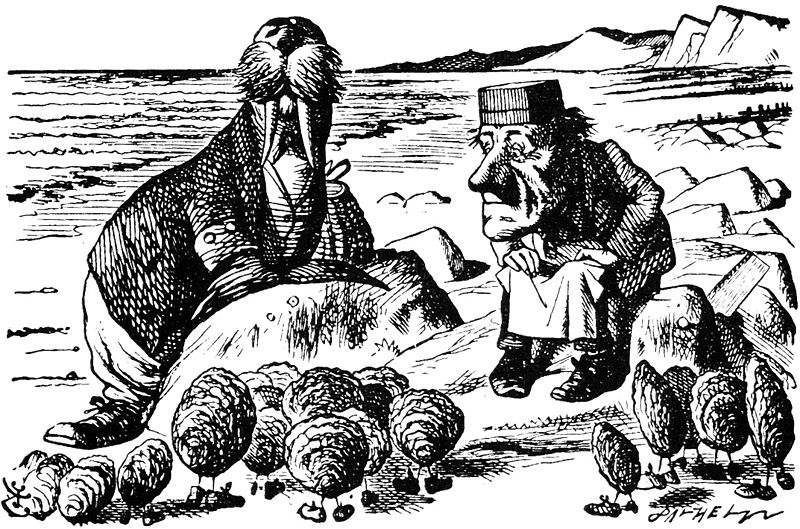
\includegraphics{images/800px-Briny_Beach.jpg}
% \end{center}
% \caption[Poem]{The Walrus and the Carpenter}
% \label{fig:walrus}
% \end{figure}

\subsection{ภาพรวมของระบบ (System Overview)}
  
ภาพรวมการทํางานของระบบนี้ จะมีส่วนการทํางานหลัก ๆ ดังนี้

• ระบบการอัพโหลดและการทํานายรอยโรคในช่องปากโดย AI

• ระบบประวัติการอัพโหลดและการทํานายรอยโรคในช่องปากสําหรับแต่ละผู้ใช้งาน

• ระบบการวงรอยโรคสําหรับทันตแพทย์(Annotation)

• ระบบการแพทย์ทางไกล (Telemedicine) สําหรับให้ความคิดเห็นระหว่างทันตแพทย์ผู้เชี่ยวชาญกับ
ทันตแพทย์ทั่วไป, อาสาสมัครสาธารณสุขประจําหมู่บ้าน, ทันตบุคลากรและผู้ใช้ทั่วไป

• ระบบจัดการผู้ใช้งาน (User Management) และระบบติดตามผู้ใช้งาน (User Tracking)

• ระบบจัดการข้อมูล (Data Management)

\subsection{โครงสร้างฐานข้อมูล (Database Schema)}

Database diagram ของระบบของเรา ได้ทําการเเบ่งผู้ใช้งานเป็น 2 ส่วนหลัก ๆ คือ patients เเละ
users โดย patients คือ คนไข้ทั่วไป เเละ users คือกลุ่มทันตเเพทย์ พนักงานสาธารณสุขเเละผู้ดูแลระบบ
รวมถึงอสม.

ตาราง comment ระบบจะให้เฉพาะทันตเเพทย์ที่มีใบ NL ในการ comment ข้อมูลเท่านั้น โดยสามารถ
บอกได้ว่าเห็นด้วยหรือไม่เห็นด้วย ด้วยเหตุผลอย่างไร

ตาราง users log เป็น table ที่สามารถดูได้เฉพาะ user ที่เป็นผู้ดูแลระบบเท่านั้น โดยจะบอกเกี่ยวกับ
action ของผู้ใช้งานทุกคนว่า ได้มีinteract กับระบบอย่างไรบ้าง โดยที่ action จะมีlogin, logout , delete
รวมถึว action ที่สําคัญต่าง ๆ ไม่ว่าจะเป็น delete user, การ uplaod image โดยเก็บเป็น unixtime เพื่อ
ทําให้ง่ายต่อการ parse

การเข้ารหัสข้อมูล (Encryption) เนื่องจากระบบของเรามีข้อมูลส่วนตัวมากมายที่เก็บเอาไว้ เราจึงต้อง
ทําการเข้ารหัสข้อมูลตาม requirement ที่เราได้รับมา โดยจะมีfile รูปภาพที่เป็นความลับของคนไข้เเละ
ทําการเข้ารหัส password เพื่อความปลอดภัย

\section{ส่วนเชื่อมต่อระหว่างผู้ใช้งานกับระบบ (User Interface)}
\subsection{ผู้ใช้งาน (User)}

\chapter{\ifproject%
\ifenglish Experimentation and Results\else การทดลองและผลลัพธ์\fi
\else%
\ifenglish System Evaluation\else การประเมินระบบ\fi
\fi}
% \chapter{\ifenglish System Evaluation\else การประเมินระบบ\fi}

ในบทนี้จะทดสอบเกี่ยวกับการทำงานในฟังก์ชันหลักๆ

\section{การทดลองเกี่ยวกับการทํางานของระบบ}

การประเมินระบบจะประเมินโดยทดสอบกับกลุ่มผู้ใช้งานทั้ง 4 กลุ่ม ได้แก่ ผู้ใช้ทั่วไป, ทันตแพทย์, ทันตบุคลากร และอาสาสมัครสาธารณสุขประจําหมู่บ้าน (อสม.) โดยในการทดสอบระบบจะมีการประเมินผลการ
ทดลองโดยใช้เกณฑ์ต่าง ๆ ดังนี้

\subsection{ผู้ใช้ทั่วไป}

ผู้ใช้ทั่วไปมักมีความต้องการใช้งานระบบที่เรียบง่าย ใช้งานง่าย ไม่ซับซ้อน ดังนั้น ในการทดสอบกับผู้ใช้ทั่วไป
ควรเน้นการประเมินปั จจัยต่างๆ เช่น

• ความน่าใช้งาน: Ease of use

• ความพึงพอใจของผู้ใช้งาน: User satisfaction


• ประโยชน์: Benefits

ตัวอย่างวิธีการทดสอบกับผู้ใช้ทั่วไป ได้แก่

• ให้ผู้ใช้ทดสอบระบบและรวบรวมข้อมูลเกี่ยวกับประสบการณ์การใช้งาน เช่น ระยะเวลาในการดําเนิน
การแต่ละขั้นตอน ความสะดวกในการใช้งาน เป็นต้น

• ให้ผู้ใช้ตอบแบบสอบถามเกี่ยวกับความพึงพอใจต่อระบบ เช่น ความง่ายในการใช้งาน ความน่าสนใจ
ของเนื้อหา เป็นต้น

• ให้ผู้ใช้ประเมินประโยชน์ที่ได้รับจากระบบ เช่น ช่วยให้ประหยัดเวลา ช่วยให้เข้าใจข้อมูลต่างๆ ได้ง่าย
เป็นต้น

\subsection{ทันตแพทย์}

ทันตแพทย์มีความต้องการใช้งานระบบที่มีประสิทธิภาพ ถูกต้องแม่นยําและสามารถช่วยในตรวจคัดกรองมะเร็งช่องปากได้อย่างมีประสิทธิภาพ ดังนั้น ในการทดสอบกับทันตแพทย์ ควรเน้นการประเมินปัจจัยต่างๆ เช่น

• ความน่าใช้งาน: Ease of use

• ความพึงพอใจของผู้ใช้งาน: User satisfaction

• ประโยชน์: Benefits

• การช่วยในการตรวจคัดกรองมะเร็งช่องปาก: Screening

ตัวอย่างวิธีการทดสอบกับทันตแพทย์ ได้แก่

• ให้ทันตแพทย์ทดสอบระบบภายใต้สถานการณ์จริง เช่น ถ่ายภาพช่องปากของผู้ป่ วย และให้ระบบตรวจ
คัดกรอง และให้ทันตแพทย์ประเมินความถูกต้องแม่นยําของระบบ เป็นต้น

• ให้ทันตแพทย์ประเมินประโยชน์ที่ได้รับจากระบบ เช่น ช่วยให้ตรวจคัดกรองมะเร็งช่องปากได้อย่างมี
ประสิทธิภาพหรือไม่ เป็นต้น

\subsection{ทันตบุคลากร}

ทันตบุคลากรมีความต้องการใช้งานระบบที่อํานวยความสะดวกในการทํางาน เช่น การดูประวัติการตรวจคัด
กรองมะเร็งช่องปาก การบันทึกข้อมูล การสรุปผลการตรวจคัดกรองมะเร็งช่องปาก ดังนั้น ในการทดสอบกับ
ทันตบุคลากร ควรเน้นการประเมินปัจจัยต่างๆ เช่น

• ความสะดวกในการใช้งาน: Ease of use

• ประโยชน์: Benefits

ตัวอย่างวิธีการทดสอบกับทันตบุคลากร ได้แก่

• ให้ทันตบุคลากรทดสอบระบบและรวบรวมข้อมูลเกี่ยวกับประสบการณ์การใช้งาน เช่น ระยะเวลาใน
การดําเนินการแต่ละขั้นตอน ความสะดวกในการใช้งาน เป็นต้น

• ให้ทันตบุคลากรประเมินประโยชน์ที่ได้รับจากระบบ เช่น ระบบช่วยให้ทํางานได้อย่างมีประสิทธิภาพ
หรือไม่ เป็นต้น

\subsection{อาสาสมัครสาธารณสุขประจําหมู่บ้าน (อสม.)}
อสม. มีความต้องการใช้งานระบบที่เข้าใจง่าย ใช้งานสะดวก และสามารถช่วยให้ให้บริการประชาชนได้อย่าง
มีประสิทธิภาพ ดังนั้น ในการทดสอบกับอสม. ควรเน้นการประเมินปัจจัยต่าง ๆ เช่น

• ความน่าใช้งาน: Ease of use

• ความพึงพอใจของผู้ใช้งาน: User satisfaction

• ประโยชน์: Benefits

ตัวอย่างวิธีการทดสอบกับอสม. ได้แก่


• ให้อสม.ทดสอบระบบและรวบรวมข้อมูลเกี่ยวกับประสบการณ์การใช้งาน เช่น ระยะเวลาในการดําเนิน
การแต่ละขั้นตอน ความสะดวกในการใช้งาน เป็นต้น

• ให้อสม.ตอบแบบสอบถามเกี่ยวกับความพึงพอใจต่อระบบ เช่น ความง่ายในการใช้งาน ความน่าสนใจ
ของเนื้อหา เป็นต้น

• ให้อสม.ประเมินประโยชน์ที่ได้รับจากระบบ เช่น ระบบช่วยให้บริการประชาชนได้อย่างมีประสิทธิภาพหรือไม่ เป็นต้น

ทั้งนี้ ในการทดสอบระบบกับผู้ใช้ทั่วไป, ทันตแพทย์, ทันตบุคลากรและอสม จะพิจารณาจากปัจจัยต่าง ๆ
เช่น วัตถุประสงค์ของการประเมิน ขอบเขตของการประเมิน ความพร้อมของระบบ เป็นต้น เพื่อให้ได้ผลการ
ประเมินที่มีประสิทธิภาพ
\ifproject
\chapter{\ifenglish Conclusions and Discussions\else บทสรุปและข้อเสนอแนะ\fi}

\section{\ifenglish Conclusions\else สรุปผล\fi}

ในการทำโครงงานนี้ สามารถพัฒนาเว็บแอปพลิเคชัน ที่สามารถทำงานร่วมกับระบบAIได้จริง
โดยมีความแม่นยำในการทำนายรอยโรคในระดับที่พึงพอใจ แต่สามารถพัฒนาให้ดียิ่งขึ้นกว่านี้ได้อีกทั้งในส่วนของ
AIและส่วนของระบบเว็บแอปพลิเคชัน ที่สามารถทำให้มีความพึงพอใจในการใช้งานมากขึ้นได้ เพิ่มให้มีความสวยงามและใช้งานง่ายขึ้น


ในส่วนของการรองรับผู้ใช้งาน ยังไม่สามารถทำได้ดีพอที่จะรองรับผู้ใช้งานหลายคนทั่วทั้งประเทศพร้อมกันได้
เนื่องจากข้อจำกัดของเซิร์ฟเวอร์ที่ใช้อยู่ในปัจจุบัน ไม่ได้มีประสิทธิภาพมากพอ และทางคณะผู้จัดทำได้วางแผนแนวทางการพัฒนาระบบ
ต่อไปในอนาคตเพื่อให้มีความเสถียรและสามารถขยายขนาด(scalability)ได้โดยไม่ใช้ทรัพยากรมากเกินจำเป็น
\section{\ifenglish Challenges\else ปัญหาที่พบและแนวทางการแก้ไข\fi}

ในการทำโครงงานนี้ พบว่าเกิดปัญหาหลักๆ ดังนี้

1. ระบบเดิมไม่ได้มีการออกแบบเพื่อรองรับการเพิ่มฟีเจอร์ใหม่ตั้งแต่แรก ทำให้การพัฒนามีความล่าช้ากว่าที่ควรเพราะต้องปรับโครงสร้างระบบใหม่
เพื่อให้การพัฒนาระบบในอนาคตเป็นไปได้อย่างราบรื่นขึ้น

2. คณะผู้จัดทำไม่ได้มีพื้นฐานความรู้ด้านการแพทย์ จึงทำให้ไม่ค่อยเข้าใจมุมมองในฐานะทันตแพทย์
ว่าต้องการให้ระบบทำอะไรได้บ้าง 

3. ในช่วงที่ทำการพัฒนาระบบอยู่ มีการใช้งานจากผู้ใช้จริงอยู่ด้วย จึงมีความเสี่ยงที่เมื่อเกิดความผิดพลาด
จะทำให้ข้อมูลจริงเสียหาย

4.ในปัจจุบันพัฒนามาเพื่อรองรับเฉพาะweb browser อาจจะทำให้การแสดงผลไม่ถูกต้องในบางอุปกรณ์ ที่มีขนาดหน้าจอไม่ตรงกับที่ระบบรองรับ

\section{\ifenglish%
Suggestions and further improvements
\else%
ข้อเสนอแนะและแนวทางการพัฒนาต่อ
\fi
}

ข้อเสนอแนะเพื่อพัฒนาโครงงานนี้ต่อไป มีดังนี้

1. ปรับโครงสร้างระบบโดยย้ายระบบไปยังcloud จะทำให้มีscalabilityและreliabilityที่สูงขึ้น

2. มีระบบbackupและrollbackฐานข้อมูล เพื่อป้องกันความผิดพลาดที่อาจจะเกิดขึ้นได้ระหว่างการพัฒนาระบบ

3. ควรมีการทำระบบอีกเวอร์ชันเพิ่มออกมาเพื่อให้ใช้ในอุปกรณ์เคลื่อนที่โดยเฉพาะ เพื่อให้ใช้งานง่าย
และสวยงามขึ้น

4. ควรเพิ่มระบบsecurityให้ดีขึ้นกว่าปัจจุบัน เพราะมีข้อมูลส่วนตัวของผู้ใช้เก็บอยู่ด้วย
อาจเกิดความเสียหายขึ้นได้เมื่อมีผู้ไม่หวังดีมาโจมตีระบบ

5. ควรมีการทำdocumentไว้เพื่อให้ผู้ที่เข้ามาพัฒนาระบบต่อไปสามารถเข้าใจได้ง่ายขึ้น


\fi

\bibliography{sampleReport}

\ifproject
\normalspacing
\appendix
\include{chapters/appendix}

%% Display glossary (optional) -- need glossary option.
\ifglossary\glossarypage\fi

%% Display index (optional) -- need idx option.
\ifindex\indexpage\fi

\begin{biosketch}
\begin{center}
  \includegraphics[width=1.5in]{mugshot.jpg}
\end{center}
Your biosketch goes here. Make sure it sits inside
the \texttt{biosketch} environment.
\end{biosketch}
\fi % \ifproject
\end{document}
